\section{Phase 2: MR Images creation}

\subsection{Variational Autoencoder}

The source code of the implemented VAE can be found at \href{https://github.com/mtablado/uoc2022_tfm/blob/main/vae.ipynb}{vae.ipynb} file inside the project repository and it is inspired by Variational Autoencoder \cite{vaekeras} keras example.

\begin{figure}[ht]
    \centering
    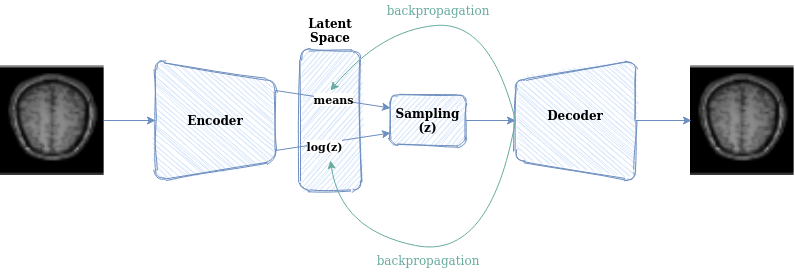
\includegraphics[width = 16cm, height = 6cm]{images/vae.png}
    \caption[]{Diagram of Implemented VAE Architecture}
    \label{fig:vaearch}
\end{figure}

The encoder consists of a \acrfull*{cnn} that uses the preprocessed brain slices images as input and then two vectors that form the latent space, which has been sized to store 1024 attributes. \acrshort*{cnn} implementation is described later in a dedicated section.

Encoder output vectors are:

\begin{itemize}
    \item A 1024-dimensional vector of means ($\mu$), and
    \item a 1024-dimensional vector of standard deviations (z) as $log(z)$ to make sure they are positive.
\end{itemize}
 
Then those vectors are sampled and feeded into the decoder to reconstruct the \acrshort{mri}. Backpropagation is applied to correct latent space issues and let the model be more accurate.

To implement above architecture in Keras, a new model was created by overriding the Keras Model abstract class and implementing the methods that the interface requires. So, specific methods are coded to process each and every train step and the metrics property is overriden to store the training loss, the reconstruction loss and the Kullback-Leibler divergence data.

The training method calculates the reconstruction loss and the KL divergence. Then, their values are aggregated to result in the training loss value.

\begin{equation}
    Training Loss = Reconstruction Loss + KL Divergence
\end{equation}

The reconstruction loss measures how close the encoder input and the encoder output are by calculating the \acrshort{mse} of the difference between images. On the other hand the KL-Divergence measures the distance between two probability distributions. So, minimizing the KL loss in this case means ensuring that the learnt means and variances are as close as possible to those of the target (normal) distribution.

The latent space of the VAE is usually a Gaussian distribution. Gaussian distribution is also used here since it has very good computational properties. 

The sampling process is implemented as an encoder Keras Layer which takes both vectors and samples with a formula that aggregates the mean and the variance which adjusted with a random factor.


\subsubsection*{The KL-Divergence issue}

As introduced in \ref*{sec:imploverview} overview section, some deviations from the project happened. The KL-Divergence interpretation and calculation was (and remains) a problem. Contrary to what should happen, instead of decreasing, the KL-Divergence metric increases along the epochs. 

Several calculation formulas for KL-Divergence were tested with little result changes (they are commented in at source file). 

The best model accuracy comes at maximizing the ELBO, which happens when you minimize both reconstruction loss and KL\-Divergence.

Despite the KL-Divergence issue, the ELBO improves in each step thanks to the higher minimization of the reconstruction loss

\begin{equation}
    \left\lvert Reconstruction Loss_i - Reconstruction Loss_{i-1} \right\rvert > \left\lvert KL Divergence_i - KL Divergence_{i-1} \right\rvert
\end{equation}
 
This casualty is allowing the model to keep learning.

This issue inclined the project to create a secondary approach, train also a \acrshort*{vqvae} model to compare results which is describe in the following section, since the time constraint did not allow the project to keep investigating on this issue.

\subsection{Vector-Quantized Variational Autoencoder}

The source code of this section can be found at \href{https://github.com/mtablado/uoc2022_tfm/blob/main/vq-vae.ipynb}{vq-vae.ipynb} file inside the project repository and it is inspired by Vector-Quantized Variational Autoencoder \cite{vqvaekeras} keras example, which code was used as starting point.

\begin{figure}[ht]
    \centering
    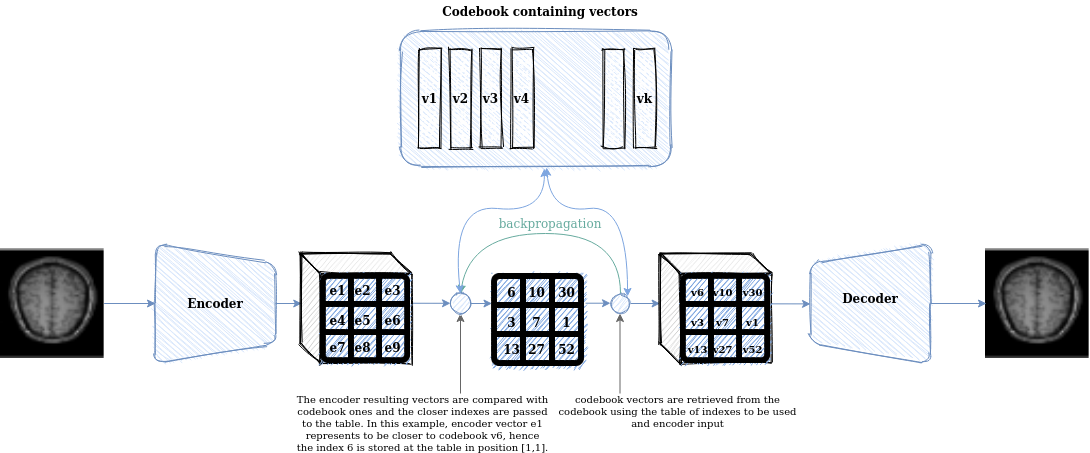
\includegraphics[width = 16cm, height = 8cm]{images/vq-vae.png}
    \caption[]{Diagram of Implemented VQ-VAE Architecture}
    \label{fig:vqvaearch}
\end{figure}

As VAE, \acrshort*{vqvae} use \acrshort*{cnn} but, in this case, the encoder generates a set of vectors with discrete representations (instead of continuous like VAE)  that is 
During training phase VQ-VAE creates a codebook of vectors which are also learnable and predictable. Once that a new image is processed, the encoder output vector of z is compared with the codebook vectors and the one closer to it is used later as the input of the decoder. Proximity between vectors is calculated with the L2-norm.

The resulting indexes are stored into a set that then serves as the indexing object to build a new set of vectors that will be used as decoder input.

To do above-mentioned steps, a Vector Quantizer object (a new type of Keras Layer) was created to select the quantized vectors from the latent space which are closer to the encoder output vectors and then, those quantized vectors will be used as decoder inputs.

To implement above architecture in Keras, as like for VAEs and along with the Vector Quantized object, a new model was created by overriding the Keras Model abstract class and implementing the methods that the interface requires. So, specific methods are coded to process each and every train step and the metrics property is overriden to store the total loss, the reconstruction loss and the VQ loss.

The training method calculates the reconstruction loss and the VQ loss and uses them to calculate the training loss (total training here) with the following formula:

\begin{equation}
    Total Loss = Reconstruction Loss + \sum (VQ losses)
\end{equation}

\subsection{CNN Network Architectures}

The implemented \acrshort{cnn} is based on Context-encoding Variational Autoencoder for Unsupervised Anomaly Detection paper \cite{cevaemodel} in where Zimmerer et al. describe it as: 

\begin{quote}
    For the encoder and decoder networks, we chose fully convolutional networks with five 2D-Conv-Layers and 2D-Transposed-Conv-Layers respectively with CoordConv, kernel size 4 and stride 2, each layer followed by a Leaky-ReLU non-linearity. The encoder and decoder are symmetric with 16, 64, 256, 1024 feature maps and a latent variable size of 1024
\end{quote}

Figure \ref{fig:cnnencoderoutput} shows the encoder model summary output after compiling the model. It is truncated to show only CNN-related layers removing VAE or VQ-VAE specific layers. Full output can be checked at Figures \ref{fig:cnnvaeencoderoutput} and \ref{fig:cnnvqvaeencoderoutput}

\begin{figure}[ht]
    \centering
    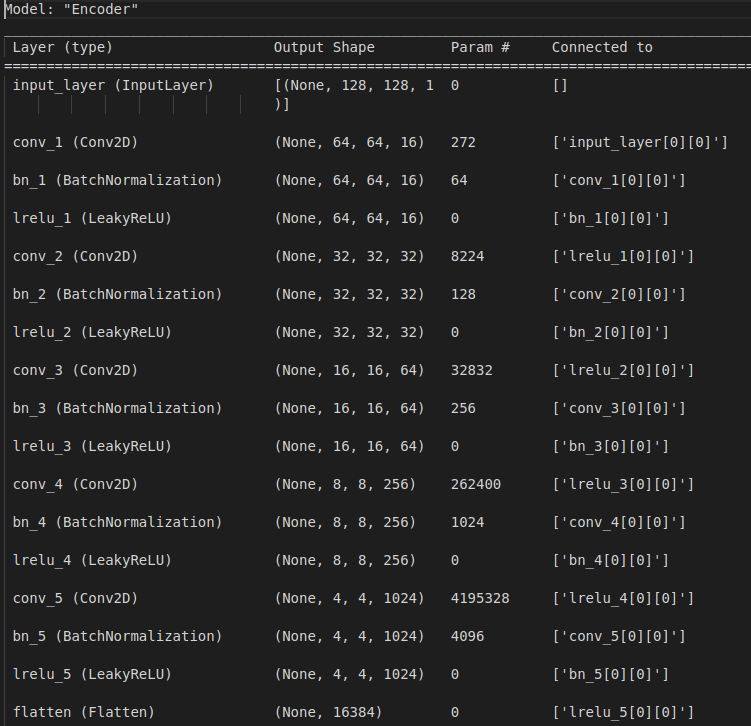
\includegraphics[width = 14cm, height = 8cm]{images/cnn-encoder-output.png}
    \caption[]{CNN Encoder model summary output}
    \label{fig:cnnencoderoutput}
\end{figure}

The input size of the \acrshort*{cnn} is [128,128,1] which are the 128 pixels resulting of the preprocessing downsampling and the usage of 1 channel for the gray scale data.

Figure \ref{fig:cnndecoderoutput} shows the decoder model summary output after compiling the model.

\begin{figure}[ht]
    \centering
    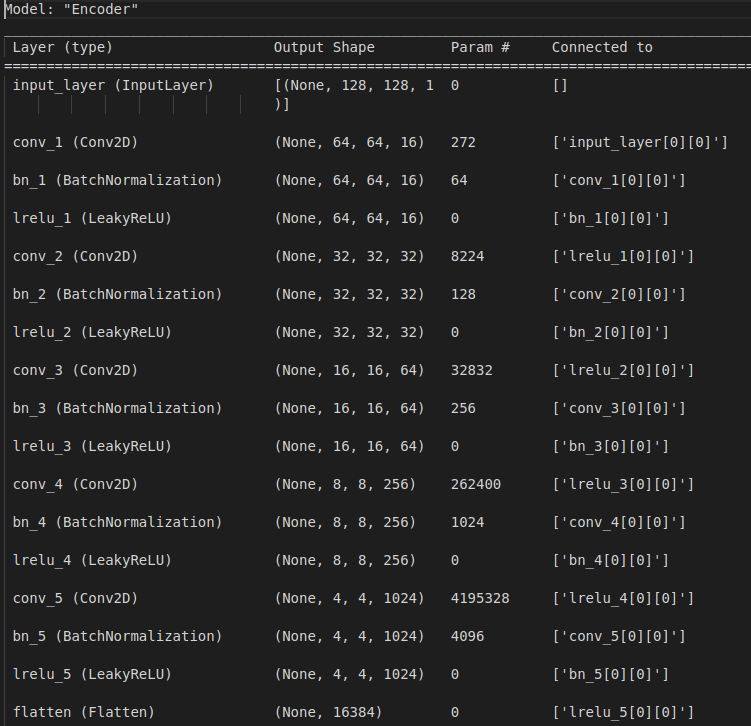
\includegraphics[width = 14cm, height = 8cm]{images/cnn-encoder-output.png}
    \caption[]{CNN Decoder model summary output}
    \label{fig:cnndecoderoutput}
\end{figure}

Both of the above-described VAE and VQ-VAE models use this network architecture to encode and decode images where different steps/layers are put in between them to implement the differences of the two models.

\newpage

\begin{figure}[ht]
    \centering
    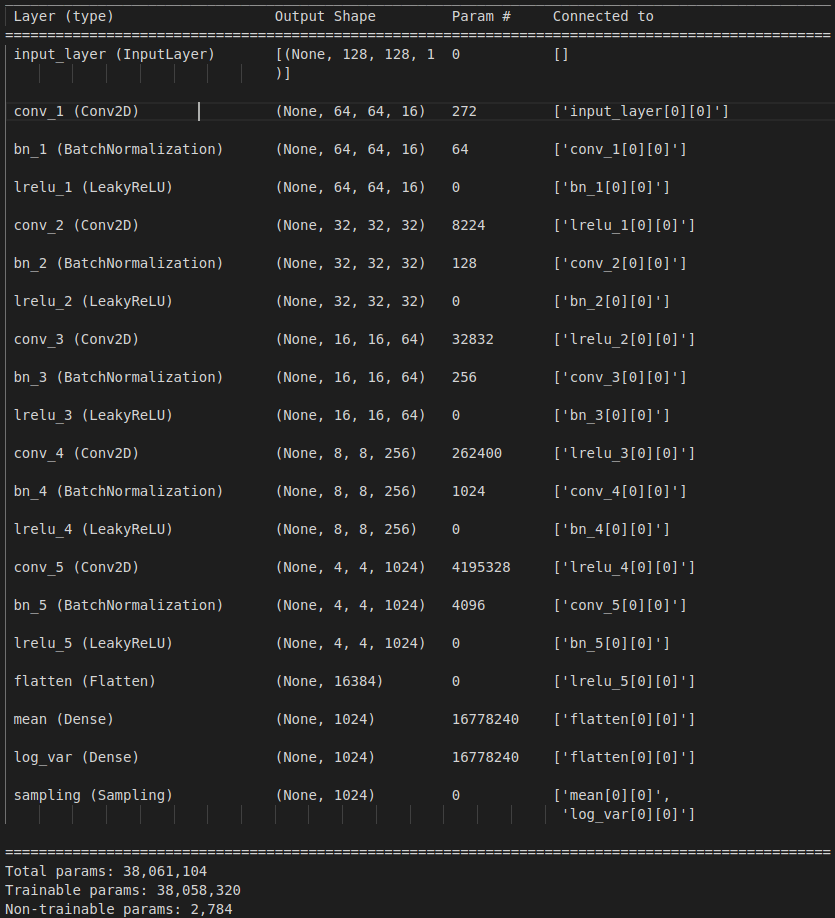
\includegraphics[width = 14cm, height = 12cm]{images/cnn-vae-encoder-output.png}
    \caption[]{CNN VAE encoder model summary output}
    \label{fig:cnnvaeencoderoutput}
\end{figure}

\newpage

\begin{figure}[ht]
    \centering
    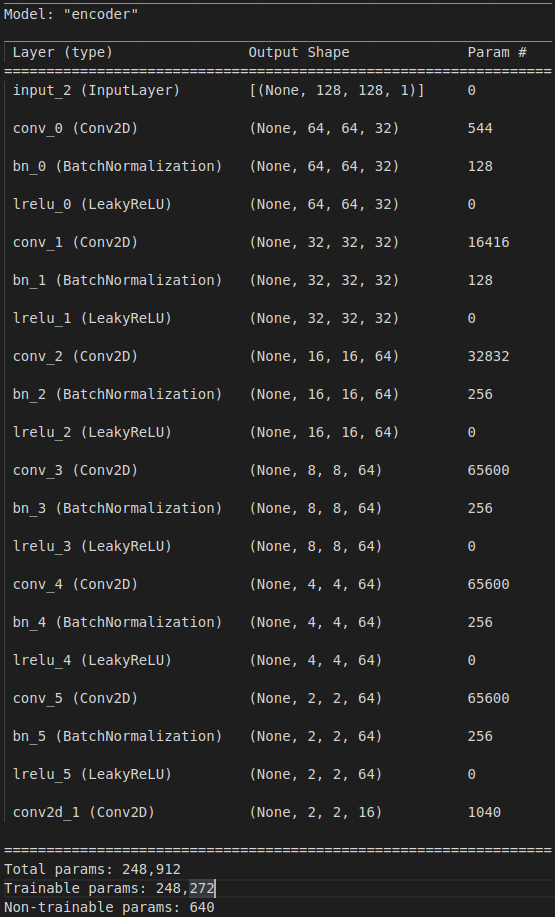
\includegraphics[width = 14cm, height = 12cm]{images/cnn-vqvae-encoder-output.png}
    \caption[]{CNN VQ-VAE encoder model summary output}
    \label{fig:cnnvqvaeencoderoutput}
\end{figure}

\subsubsection{Hidden Layers}

As described in this section, the implemented \acrshort{cnn} is based on Context-encoding Variational Autoencoder for Unsupervised Anomaly Detection paper \cite{cevaemodel} in where Zimmerer et al. describe it as: 

\begin{quote}
    For the encoder and decoder networks, we chose fully convolutional networks with five 2D-Conv-Layers and 2D-Transposed-Conv-Layers respectively with CoordConv, kernel size 4 and stride 2, each layer followed by a Leaky-ReLU non-linearity. The encoder and decoder are symmetric with 16, 64, 256, 1024 feature maps and a latent variable size of 1024
\end{quote}

In project's \acrfull{cnn}, a Normalization neuron is added between them resulting in the following composite:

\begin{itemize}
    \item Convolutional neuron (Conv2D or Conv2DTranspose) 
    \item Normalization neuron (BatchNormalization)
    \item ReLu neuron (LeakyReLu)
\end{itemize}

The convolutional layer is paremetrized with 4 kernels, stride 2 and padding 0. The kernel size aims to avoid the network learning too fast, while using stride 2 to lower the training resources needed and train faster.

According to Martin Riva \cite{batchnorm} "Batch Norm is a normalization technique done between the layers of a Neural Network instead of in the raw data. It is done along mini-batches instead of the full data set. It serves to speed up training and use higher learning rates, making learning easier. the standard deviation of the neurons' output.". The project is loading raw data in batches which are normalized as a preparation step, however, normalizing data between each layer might help.

ReLu neuron is usually applied in Deep Learning (and so it is in the project) right after every convolutional neuron to remove linearity since, basically, all the previous operations are linear. 

\subsection{Flow from directory}

An interesting implemented feature is the ability to use an interator for image loading which is in fact called by the VAE and VQ-VAE models. So that in each iteration a batch of images is loaded in memory and ready to be used within the model.

Aligning the model batch size with the iterator batch size avoids unnecessary calls and more importantly tunes memory usage while training the models.

The flow from directory method is also the responsible to downsample pixeling since images are stored with 256 and the model expects only 128.

\subsection{Creating artificial images from latent space}

To create artificial images from the latent space the decoder input must be generated. As explained, the decoder expects an object from the latent space, which means that 1024 values are expected in the normal Gaussian distribution. This is randomly generated with NumPy library and its \href{https://numpy.org/doc/stable/reference/random/generated/numpy.random.normal.html}{numpy.random.normal} function.